\chapter{Implementation and Results}\label{Implementation and Results}

\section{LOF}
We have used a synthetic 2-D dataset with 3 clusters of varying density to implement and verify LOF.
Dataset description\\
No of attributes : 2\\
No of instances  : 1500\\
No of clusters   : 3\\
Cluster 1        :  750 points in range [600,1000] \\
Cluster 2        :  500 points in range [200,450] \\
Cluster 3        :  200 points in range [0,100] \\
Noisy points	 : 50

\begin{figure}[h!]
	\centering
	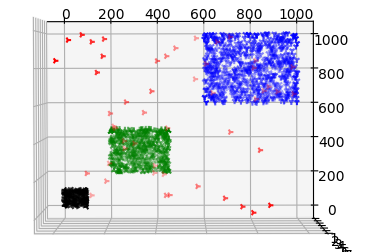
\includegraphics{chap03/LOF_dataset.png}
	\caption{2-D Dataset used for LOF}
\end{figure}

It can be seen from Figure 3.2 that points inside a cluster has LOF values nearly equal to 1 where as noisy points have LOF up to 7. More the LOF score more is the degree of anomaly.

\begin{figure}[h!]
	\centering
	\includegraphics{chap03/LOF_result.png}
	\caption{LOF values for synthetic 2-D dataset}
\end{figure}



  

